\documentclass[11pt,]{article}
\usepackage{lmodern}

\usepackage{amssymb,amsmath}
\usepackage{ifxetex,ifluatex}
\usepackage{fixltx2e} % provides \textsubscript
\ifnum 0\ifxetex 1\fi\ifluatex 1\fi=0 % if pdftex
  \usepackage[T1]{fontenc}
  \usepackage[utf8]{inputenc}
\else % if luatex or xelatex
  \ifxetex
    \usepackage{mathspec}
    \usepackage{xltxtra,xunicode}
  \else
    \usepackage{fontspec}
  \fi
  \defaultfontfeatures{Mapping=tex-text,Scale=MatchLowercase}
  \newcommand{\euro}{€}
\fi
% use upquote if available, for straight quotes in verbatim environments
\IfFileExists{upquote.sty}{\usepackage{upquote}}{}
% use microtype if available
\IfFileExists{microtype.sty}{%
\usepackage{microtype}
\UseMicrotypeSet[protrusion]{basicmath} % disable protrusion for tt fonts
}{}
\usepackage[lmargin=5cm,rmargin=2.5cm,tmargin=2.5cm,bmargin=2.5cm]{geometry}

%% citation setup

\usepackage{csquotes}

\usepackage[backend=biber, maxbibnames = 99, style = apa]{biblatex}
\setlength\bibitemsep{1.5\itemsep}
\addbibresource{R_packages.bib}
\bibliography{references.bib}
\usepackage{longtable,booktabs}
\usepackage{graphicx}
\makeatletter
\def\maxwidth{\ifdim\Gin@nat@width>\linewidth\linewidth\else\Gin@nat@width\fi}
\def\maxheight{\ifdim\Gin@nat@height>\textheight\textheight\else\Gin@nat@height\fi}
\makeatother
% Scale images if necessary, so that they will not overflow the page
% margins by default, and it is still possible to overwrite the defaults
% using explicit options in \includegraphics[width, height, ...]{}
\setkeys{Gin}{width=\maxwidth,height=\maxheight,keepaspectratio}
\ifxetex
  \usepackage[setpagesize=false, % page size defined by xetex
              unicode=false, % unicode breaks when used with xetex
              xetex]{hyperref}
\else
  \usepackage[unicode=true]{hyperref}
\fi
\hypersetup{breaklinks=true,
            bookmarks=true,
            pdfauthor={Jonathan Berrisch, Timo Rammert},
            pdftitle={A Forecasting Study on Global Wine Sales},
            colorlinks=true,
            citecolor=blue,
            urlcolor=blue,
            linkcolor=magenta,
            pdfborder={0 0 0}}
\urlstyle{same}  % don't use monospace font for urls
\setlength{\parindent}{0pt}
\setlength{\parskip}{6pt plus 2pt minus 1pt}
\setlength{\emergencystretch}{3em}  % prevent overfull lines
\setcounter{secnumdepth}{5}

%%% Use protect on footnotes to avoid problems with footnotes in titles
\let\rmarkdownfootnote\footnote%
\def\footnote{\protect\rmarkdownfootnote}

%%% Change title format to be more compact
\usepackage{titling}

% Create subtitle command for use in maketitle
\newcommand{\subtitle}[1]{
  \posttitle{
    \begin{center}\large#1\end{center}
    }
}

\setlength{\droptitle}{-2em}
  \title{A Forecasting Study on Global Wine Sales}
  \pretitle{\vspace{\droptitle}\centering\huge}
  \posttitle{\par}
\subtitle{Statistical Learning}
  \author{Jonathan Berrisch, Timo Rammert}
  \preauthor{\centering\large\emph}
  \postauthor{\par}
  \predate{\centering\large\emph}
  \postdate{\par}
  \date{today}


%% linespread settings

\usepackage{setspace}

\onehalfspacing

% Language Setup

\usepackage{ifthen}
\usepackage{iflang}
\usepackage[super]{nth}
\usepackage[ngerman, english]{babel}

% Multicols for the Title page
\usepackage{multicol}

\begin{document}

\selectlanguage{english}


%\maketitle

\begin{titlepage}
  \noindent\begin{minipage}{0.6\textwidth}
	  \IfLanguageName{english}{University of Duisburg-Essen}{Universität Duisburg-Essen}\\
	  \IfLanguageName{english}{Faculty of Business Administration and Economics}{Fakultät für Wirtschaftswissensschaften}\\
	  \IfLanguageName{english}{Chair of Econometrics}{Lehrstuhl für Ökonometrie}\\
  \end{minipage}
	\begin{minipage}{0.4\textwidth}
	  \begin{flushright}
  	  \vspace{-0.5cm}
      \IfLanguageName{english}{\includegraphics*[width=5cm]{Includes/duelogo_en.png}}{\includegraphics*[width=5cm]{Includes/duelogo_de.png}}
	  \end{flushright}
	\end{minipage}
  \\
  \vspace{1.5cm}
  \begin{center}
  \huge{A Forecasting Study on Global Wine Sales}\\
  \vspace{.25cm}
  \Large{Statistical Learning}\\
  \vspace{0.5cm}
  \large{Term Paper}\\
  \vspace{1cm}
  \large{
  \IfLanguageName{english}{Submitted to the Faculty of \\ Business Administration and Economics \\at the \\University of Duisburg-Essen}{Vorgelegt der \\Fakultät für Wirtschaftswissenschaften der \\ Universität Duisburg-Essen}\\}
  \vspace{0.75cm}
  \large{\IfLanguageName{english}{from:}{von:}}\\
  \vspace{0.5cm}
  Jonathan Berrisch, Timo Rammert\\
  \end{center}
  %\vspace{2cm}
  \vfill
  \hrulefill

  \noindent\begin{minipage}[t]{0.3\textwidth}
  \IfLanguageName{english}{Reviewer:}{Erstgutachter:}
  \end{minipage}
  \begin{minipage}[t]{0.7\textwidth}
  \hspace{1cm}Dr.~Thomas Deckers
  \end{minipage}

  \noindent\begin{minipage}[t]{0.3\textwidth}
  \IfLanguageName{english}{Deadline:}{Abgabefrist:}
  \end{minipage}
  \begin{minipage}[t]{0.7\textwidth}
  \hspace{1cm}Aug.~27th 2019
  \end{minipage}

  \hrulefill

  \begin{multicols}{3}

  Name:

  Matriculation Number:

  E-Mail:

  Study Path:

  Semester:

  Graduation (est.):

  \columnbreak

  Jonathan Berrisch

  3071485

  Jonathan@Berrisch.biz

  M.Sc. Economics

  \nth{4}

  Summer Term 2020

  \columnbreak

  Timo Rammert

  3030862

  t.rammert03@gmail.com

  M.Sc. Economics

  \nth{2}

  Winter Term 2020/2021

  \end{multicols}

\end{titlepage}


\pagenumbering{Roman}
{
\hypersetup{linkcolor=black}
\setcounter{tocdepth}{3}
\tableofcontents
}
\newpage
\listoftables
\addcontentsline{toc}{section}{List of Tables}
\newpage
\listoffigures
\addcontentsline{toc}{section}{List of Figures}
\newpage
\pagenumbering{arabic}
\hypertarget{introduction}{%
\section{Introduction}\label{introduction}}

This paper presents a forecasting study on global wine sales. This study
is based on the friberg gronqvist wine data set which is publicly
available and was previously analyzed by
\textcite[][p. 193f.]{Friberg2012}. Recent technological advancements
led to a significant increase in statistical methods that are
computationally demanding while potentially outperforming classical
statistical methods, especially in terms of forecasting. Those
techniques are usually reffered as statistical- or machine learning
methods.

We present various models which are increasingly complex. Those models
potentially gain forecasting power while losing interpretability. The
applied models range from linear regressions to tree based methods like
random forests and boosting. The goal is to develop the best possible
model to forecast weekly wine sales in litre in out of sample data.

Although the main goal is an accurate forecast, some of the methods used
in this paper can also be used to quantify the impact of expert reviews
on the sales, if there is any. The effect of expert opinions on consumer
demand was analyzed in preceeding research. Notably,
\textcite[][p. 1289]{Hilger2011} used a field experiment to study a
review-based demand effect using wine score labels in a retail grocery
chain. They find that providing information based on expert opinions
increases the sales; this effect does depend on the score a wine has
gotten. \textcite[][p. 293]{Ashenfelter2013} analyze, wether expert
reviews influence the prices of wine. They conclude, that expert reviews
contain public as well as private information. They only validate an
influence on the highest rated wines. Furthermore,
\textcite[][p. 182f.]{Bicknell2012} delivered research concerning the
market for wine from new zealand. They validate a significant regional
influence on wine prices. This influence is substantially lower for wine
which is designated for the export market.

The remainder of this paper is structured as follows. Chapter 2 gives an
overview about the dataset and the preprocessing. Chapter 3 describes
the validation approach. Chapter 4 presents the models and their
specification. Chapter 5 provides the results, a conclusion and some
ideas for future research.

\hypertarget{data-and-variables}{%
\section{Data and Variables}\label{data-and-variables}}

The data set used in this paper contains 145179 observations with 59
variables. The variables include the name of the wine, the country of
origin, its price, the amount sold per week in litre, the taste segment
and variables related to different reviews among others. We need to omit
two variables beforehand, namely \enquote{time\_segm\_price} and
\enquote{artikpr}, because those are combinations of other existing
variables. Hence inclusion would lead to the problem of
multicollinearity. After omitting those two we have left the following
types of variables:

\begin{longtable}[]{@{}rrrr@{}}
\caption{Frequency of Variable Types.}\tabularnewline
\toprule
Date & factor & logical & numeric\tabularnewline
\midrule
\endfirsthead
\toprule
Date & factor & logical & numeric\tabularnewline
\midrule
\endhead
1 & 8 & 19 & 29\tabularnewline
\bottomrule
\end{longtable}

Figure 1 depicts the amount of missing values in each variable. The
number of complete cases would be zero without further selection.
Therefore we exclude every variable with a ratio of missing values that
exceeds \(50\%\). In consequence 41416 observations with 45 variables
are used for building the forecasting models.

\begin{figure}
\centering
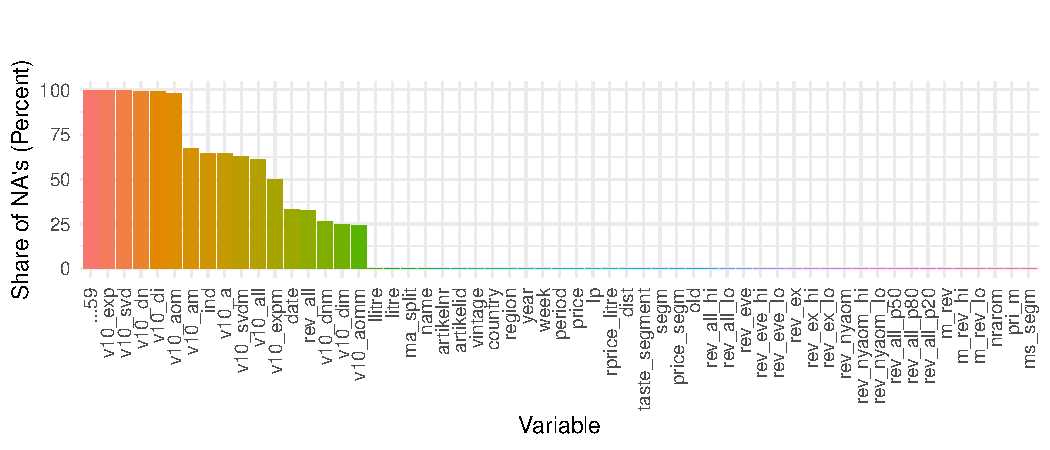
\includegraphics{../00_data/output_paper/02_missings_alt.pdf}
\caption{Share of Missing Values in the Wine Dataset.}
\end{figure}

Figure XY depicts the distribution of the litre variable which is the
dependend variable in our models. One can see that the observations are
heavily skewed. The Maximum is at \(184200\) litres sold weekly while
it's minimum is near zero with only \(0.75\) litres sold per week.

\begin{figure}
\centering
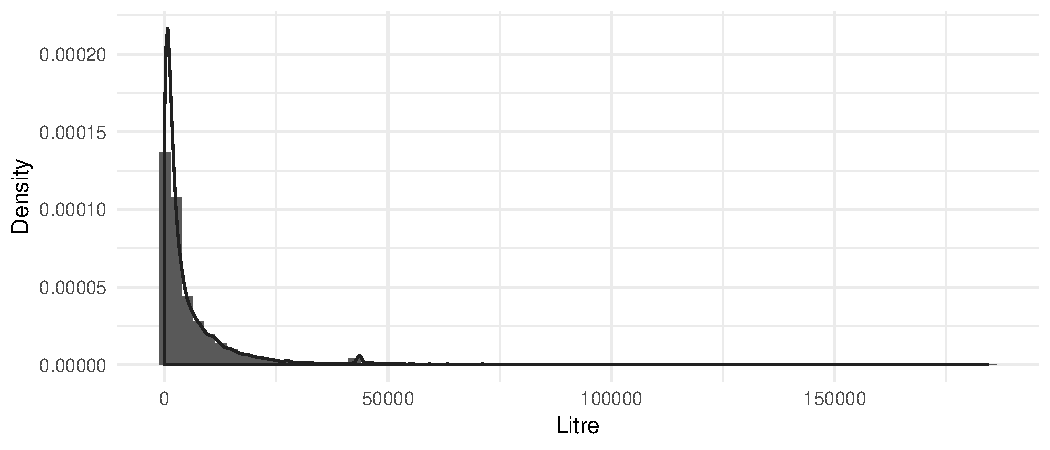
\includegraphics{../00_data/output_paper/04_hist_litre.pdf}
\caption{Histogram and Estimated Density of the Litre Variable.}
\end{figure}

\hypertarget{validation-approach}{%
\section{Validation Approach}\label{validation-approach}}

Sampling may influence the model selection process because a sample
could be in favor of one specific method while another sample could lead
to different results. Therefore we validate the results of each method
using a 5-fold cross-validation. This reduces the influence of sampling
when building a training and test set while it's computationally
feasible.

In order to compute a prediction it is necessary that the test set
includes, at least, all features of the training set. Due to the high
number of levels in the countries and name variable this was not always
the case. Therefore, we are using only the intersection of training and
test features to be included in the estimation.

\hypertarget{analysis}{%
\section{Analysis}\label{analysis}}

\hypertarget{mean-regression-and-linear-regression}{%
\subsection{Mean Regression and Linear
Regression}\label{mean-regression-and-linear-regression}}

At first a mean regression and a linear regression are calculated. Those
models are representing the baseline. For comparison of the different
models, the Root Mean Sqaured Error (RMSE)
\[\sqrt{\frac{1}{n}\sum_{i = 1}^{n}\left(y_i-\hat{y}_i\right)^2}\] is
calculated.

The mean regression yields an average RMSE of \(\approx 13340\) litre
sold per week. The linear regression where all variables are included
yields an average RMSE of \(\approx 5572\). The latter result is
probably influenced by overfitting. To cope with this problem, we are
using variable selection and dimension reduction methods which are
discussed in the proceeding sections.

\hypertarget{lasso}{%
\subsection{Lasso}\label{lasso}}

The Least Absolute Shrinkage and Selection Operator (Lasso) is a method
combining linear regression and shrinkage of the coefficent estimates to
do variable selection. It fits a linear model that is constrained by a
penalty term, i.e., the lasso coefficients minimize:

\[
\sum_{i=1}^{n}(y_i - \beta_0 - \sum_{j=1}^{p}\beta_jx_{ij})+\lambda\sum_{j=1}^{p}|\beta_j|.
\]

Figure XY depicts the relation between lambda and the coefficients. The
crossvalidated log lambda, which minimizes the test error is
\(\approx -8.94\). At that level a total of \(\approx 666\) out of
\(713\) coefficients are
nonzero\footnote{$\approx 666.6$ to be exact, but we couldn't resists to round down.}.
The other coefficients are exactly zero due to the sparsitiy property of
the lasso estimator. Furthermore, the plot includes abbreviated variable
names of the 10 biggest coefficients. All of those coefficients are
dummys for specif*ic wine names. The average RMSE of the lasso approach
is \(\approx 5547.76\). This is a slight improvement compared to the
linear baseline model. The lasso slightly reduces the feature set while
also reducing the RMSE. This is evidence supporting our prior assimption
that the linear model was exposed to the problem of overfitting.
Furthermore, the coefficients of the lasso model show that the name
variable is the most important variable to explain the sold litre per
week. It is followed by the Vintage, the Region, the taste segment and
the Country of the wine. The least important variables are the review
variables which are not present in the 400 biggest coefficients.

\begin{figure}
\centering
\includegraphics{term_paper_files/figure-latex/unnamed-chunk-6-1.png}
\caption{Relation of Coefficients and Shrinkage.}
\end{figure}

\hypertarget{pcr-and-pls}{%
\subsection{PCR and PLS}\label{pcr-and-pls}}

While lasso is a technique for variable selection, PCR (principal
components regression) and PLS (partial least squares) are methods that
reduce the dimension of the feature set. Thus, the least squares
estimation is performed using a transformation of the explanatory
variables. Thereby, PLS includes the dependent variable when computing
the new feature set while PCR builds the principal components
independent of the dependent variable.

Figure XY shows the first two principal components from a principal
components analysis. The first two principal components represent
roughly 3\% of the total variance. This is a sign that the PCA doesn't
work well in our data which might be due to the large amount of dummy
variables.

\begin{figure}
\centering
\includegraphics{term_paper_files/figure-latex/unnamed-chunk-8-1.png}
\caption{Principal Component One and Two.}
\end{figure}

The results confirm the expectation. PCR has a cross-validated RMSE of
\(\approx 5546.05\) while PLS leads to an RMSE of \(\approx 6201.15\).
While \(\approx 635\) principal component where included in the PCR,
only \(\approx 35.2\) components where used in the PLS. Thus PLS
significantly reduced the dimension of the featureset. While sacrificing
interpretability of the results, it leads to a higher RMSE.

\hypertarget{splines}{%
\subsection{Splines}\label{splines}}

The previous methods assumed linear relationships between the
independent variables and the dependent variable. Considering the amount
of dummy variables in the feature set the usage of nonlinear methods is
quite limited. However, to recognize potential nonlinear relationships
we add natural splines to the \(year\), \(price\), and \(rprice\_litre\)
variable. Those variables indicate the year in which the wine was
distributed, the price and the real price with Jan 2004 as base
respectively. Each natural spline was allowed to have up to 20 knots
which is sufficient to estimate complex linear relationships. The
respective RMSEs depending on the knots are presented in figure
\ref{fig:splines}. Splines are able to improve the prediction a little
which indicates that at least some nonlinear relationship is present.
However, like the methods before, splines reduce the interpretability of
the coefficients. In this case, this tradeoff isn't offset enough by the
gain in precision. Furthermore, figure \ref{fig:splines} shows, that the
RMSEs depend to some extend on the fold which was used for
cross-validation. This approves our theoretically founded motivation to
use cross-validation.

\begin{figure}

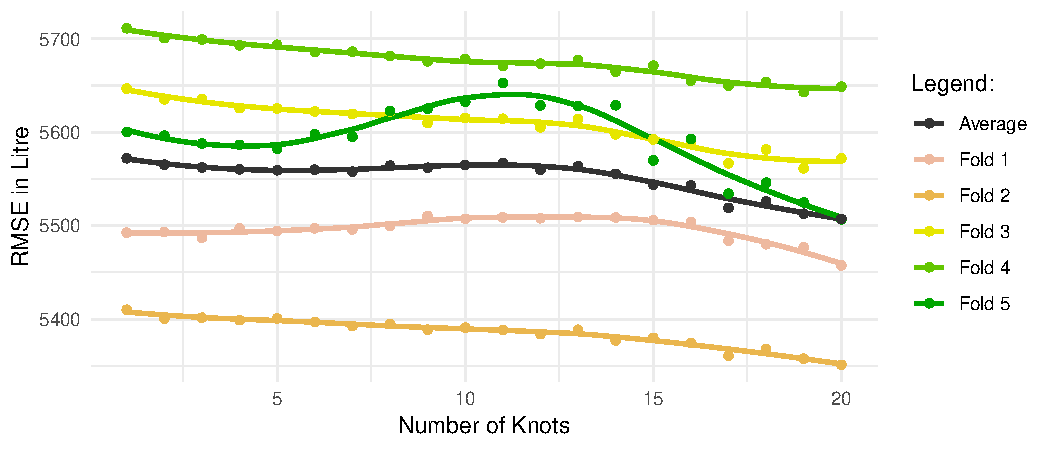
\includegraphics{../00_data/output_paper/08_splines} \hfill{}

\caption[RMSE Values of Different Spline Models]{\label{fig:splines}Regression with Splines: Dependency Between Knots and RMSE.}\label{fig:splines}
\end{figure}

\hypertarget{decision-tree-methods}{%
\subsection{Decision tree methods}\label{decision-tree-methods}}

Tree-based methods utilze decision rules to split the feature space into
a number of different regions. `Since the set of splitting rules used to
segment the predictor space can be summarized in a tree, these type of
approaches are known as decision tree methods'
\autocite[][p. 303]{Hastie2013}. The base of tree-based methods are
regression trees For improvement of the predictive power of these
methods, while losing interpretability, one can combine different
regression trees for a single prediction. Those approaches, including
bagging, random forests and boosting, are described in more detail when
being applied.

\hypertarget{regression-tree}{%
\subsubsection{Regression Tree}\label{regression-tree}}

For growing a regression tree `the algorithm needs to automatically
decide on the splitting variables and split points {[}\ldots{}{]} the
tree should have' \autocite[][p. 349]{Hastie2013}. The tree is grown
when a splitting is found that minimizes the sum of squared residuals.
The splitting is done with a greedy algorithm, i.e., at first all the
data is split into just two groups while the search of the splitting
variable and split point includes all possible variables and points
\autocite[cf.][p. 349]{Hastie2013}. After the data is split this process
is repeated for the now obtained two splitted regions until the tree is
large enough that the nodes reach a set minimum size.

\begin{figure}
\centering
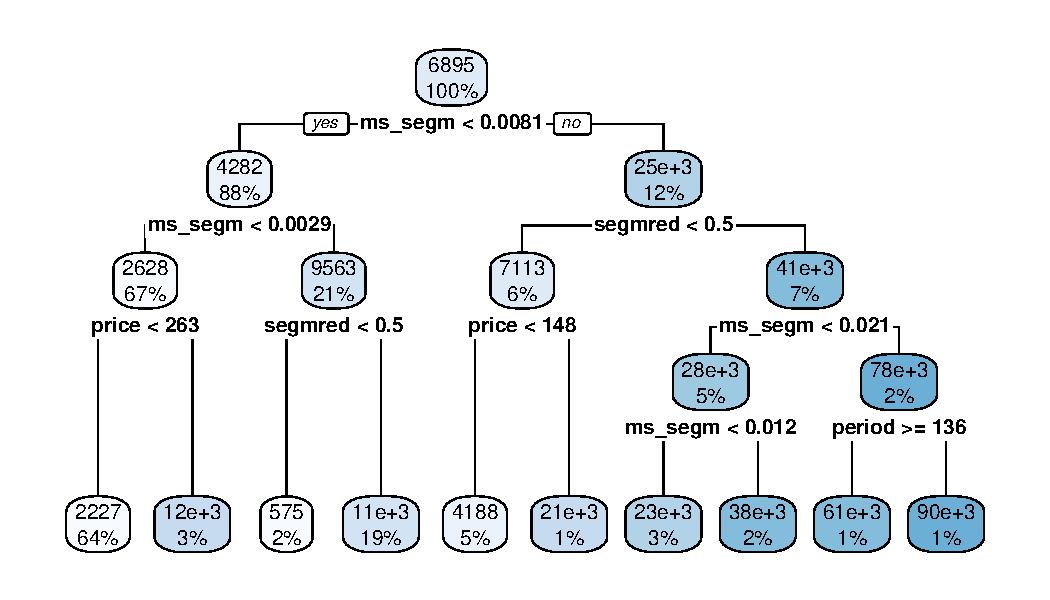
\includegraphics{../00_data/output_paper/09_tree.pdf}
\caption{\label{fig:tree}Example of a Regression Tree.}
\end{figure}

Figure \ref{fig:tree} shows that only a few of the available variables
are used. These are namely \(ms\_segm\), \(segmred\), \(price\), and
\(period\) and split the dataset into \(10\) parts, i.e., the tree has
got \(10\) terminal nodes. The figure does also tell us what share of
the data can be sorted to each node, as well as the mean price of the
allocated observations. The regression trees build in the other four
folds of the cross-validation are almost exactly the same as the shown
tree. The selected variables indicate that according to this method the
market share, the color of the wine, the price as well as the period.
Concerning the graph and the variable \(segmred\) it is important to
keep in mind that this is a dummy variable meaning that a value
\(< 0.5\) (the left track) stands for a wine that isn't red. Conversely
the right track stands for red wines.

As regression trees may tend to grow quite large, a possible way to get
smaller trees is pruning back the grown larger tree. The goal of pruning
is `to select a subtree that leads to the lowest test error rate
{[}which{]} we can estimate {[}\ldots{}{]} using cross-validation or the
validation set approach' \autocite[][p. 308]{James2014}. This is done by
\emph{cost complexity pruning}.

\begin{figure}
\centering
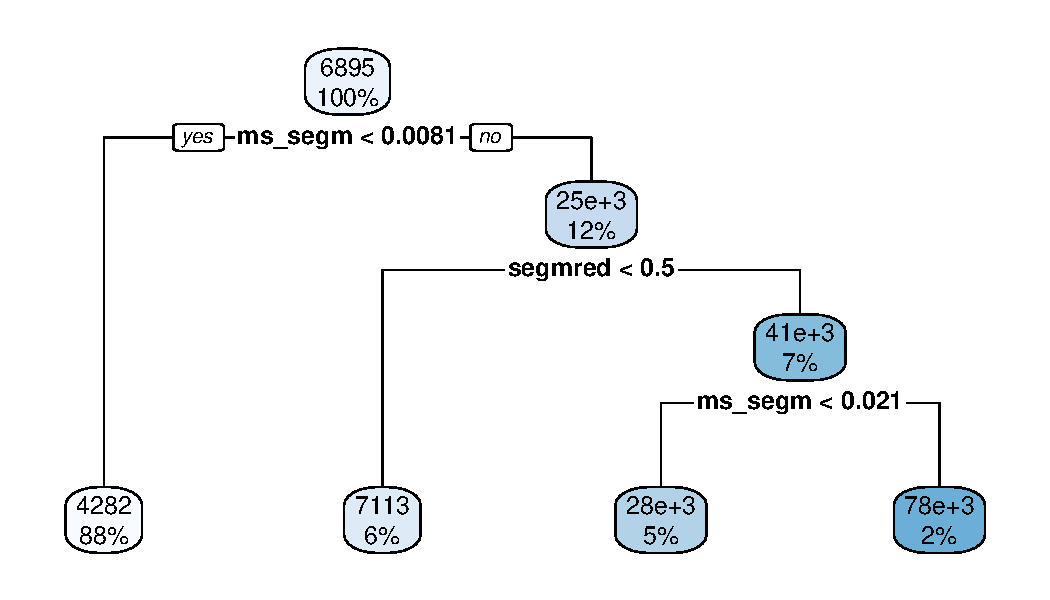
\includegraphics{../00_data/output_paper/09_tree_pruned.pdf}
\caption{\label{fig:tree_pruned}Example of a Pruned Tree.}
\end{figure}

The pruned tree (see Figure \ref{fig:tree_pruned}) does only utilze the
dummy whether the wine is a red wine and the mean market share within
color during weeks the wine is distributed. \(ms\_segm\) is used twice
and thus the pruned tree splits the data set into four terinal nodes.
While the pruned tree thus might be easier to interpret, it does also
come with a higher RMSE. The mean cross-validated RMSE of the pruned
trees is ca. 7935.64, while the mean RMSE of the normal regression trees
is about 6494.75.

\hypertarget{bootstrap-aggregation}{%
\subsubsection{Bootstrap Aggregation}\label{bootstrap-aggregation}}

Bootstrap aggregation (Bagging) is a general method of repeatedly taking
bootstrap samples from the dataset, estimating a model for every sample
and averaging the predictions of every model afterwards. The bagging
algorithm can also be used to improve decision tree models. For this, a
bootstrap sample is drawn before growing the tree. This process is
repeated several times to grow multiple trees. Finally, the predictions
of the trees are averaged. By bootstrapping bagging brings down the
variance and thus, adresses the main problem of single regression trees
which are very dependent on the actual sample.

Figure \ref{fig:rmsebag} shows the RMSE values of different bagging
models. The bootstrap sample size was chosen to be two thirds of the
total number of observations. One can see that even small models with
down to 15 Trees significantly outperform the single tree model of the
previous chapter.

\begin{figure}

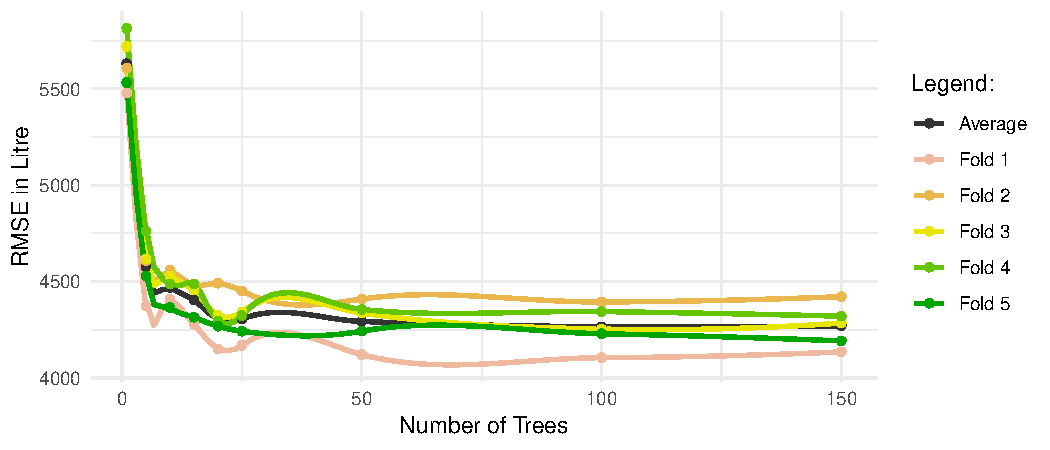
\includegraphics{../00_data/output_paper/14_bagging} \hfill{}

\caption[Bagging: RMSE's at Different Tree Sizes]{\label{fig:rmsebag}Bagging: RMSE's at Different Tree Sizes (Smoothed).}\label{fig:bag}
\end{figure}

To further analyze the bagging model, we estimated a bagging model with
25 trees for the whole dataset. Figure \ref{fig:bagvarimp} is a variable
importance plot for this model. It presents those 20 variables which
would increase the RMSE the most when being omitted. The plot shows that
the influence of \enquote{ms\_segm} which is the market share of the
wine as well as \enquote{segmred} which is a dummy, indicating if the
whine is red, substantially contribute to our model. Intuitively, the
price also influences how many litres per week are sold. More
surpisingly however is the fact, that also the date substantially
contributes to our mode. This indicates that prices have changed oder
time.

\begin{figure}

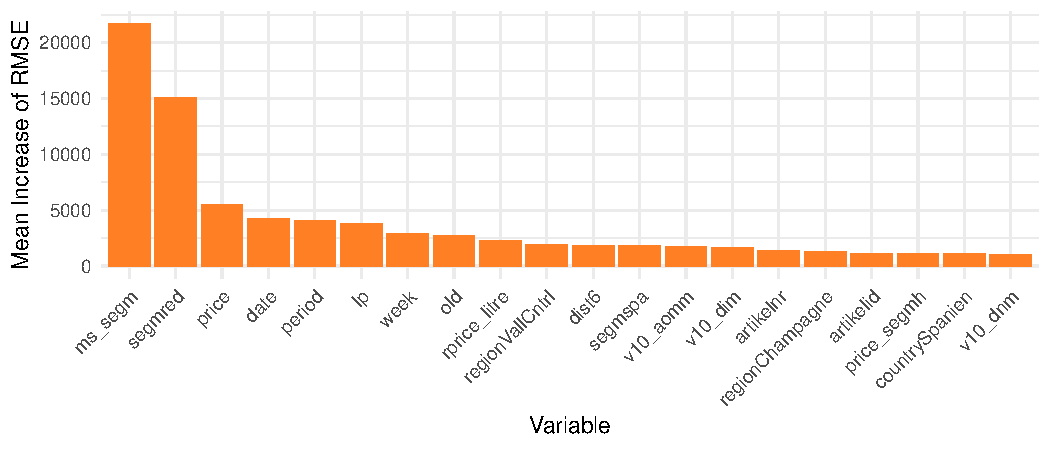
\includegraphics{../00_data/output_paper/15_var_imp_bagging} \hfill{}

\caption{\label{fig:bagvarimp}Bagging: Variable Importance.}\label{fig:bag_varimp}
\end{figure}

Bagging, in general, takes all possible variables into consideration at
each split. This makes bagging computationally demanding. Moreover, this
may lead to similar trees at each iteration. Thus, the trees are
probably highly correlated.

\hypertarget{random-forest}{%
\subsubsection{Random Forest}\label{random-forest}}

The Random Forest algorithm is a special case of Bagging. The name
random forest arises from the fact that, in cotrast to the usual Bagging
algorithm, at each split of the tree building process only a pre
specified number of randomly chosen variables are taken into
consideration. This results in a different tree for each iteration off
the random forest and therefore decorrelates the trees. In consequence,
the Random Forest reduces the overall variance in comparison to Bagging.
This effect is especially valid for homogenous datasets in which the
trees of the bagging algorithm are highly correlated.

\begin{figure}

{\centering 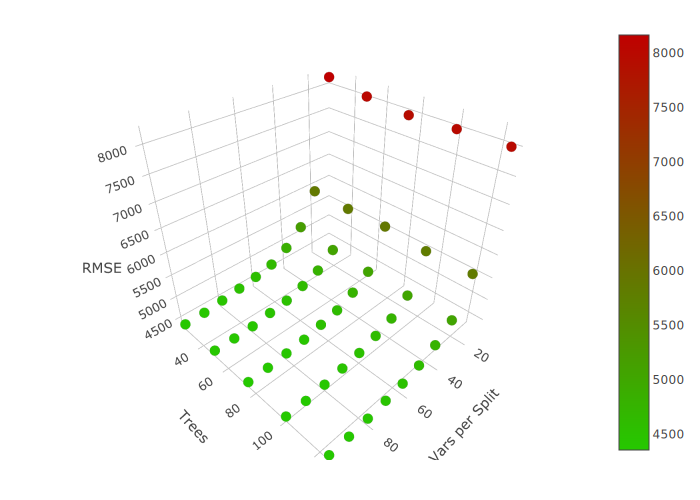
\includegraphics{../00_data/output_paper/10_rf_plot} 

}

\caption[RMSE's of the Random Forest for Different Parameters]{\label{fig:rfrmse}Random Forest: Dependency between RMSE, the Number of Trees and the Number of Variables Included at each Split.}\label{fig:unnamed-chunk-10}
\end{figure}

We calculated RMSE values for a range of Random Forest models to
evaluate which combination of the number of trees to grow and the number
of variables taken into account at each split leads to the best results.
The results are plotted in Figure \ref{fig:rfrmse}. The smallest RMSE is
\(\approx 4374\). Moreover, the plot shows, reveals, that very small
models profit substantially from increasing complexity while bigger
models profit only by a small margin. The model with 20 Trees and 80
Variables at each split still has a RMSE of \(\approx 4456\), which is
an increase of less than \(1.9\%\).

The 25 Tree Bagging Model (RMSE of \(\approx 4305\)) outperforms the
Random Forest Model (with 25 Trees and 100 Variables) only by a small
margin (RMSE of \(4374.330\)). However, training the Random Forest
demands only \(15\%\) of the time, that the Bagging Model needs.

\begin{figure}
\centering
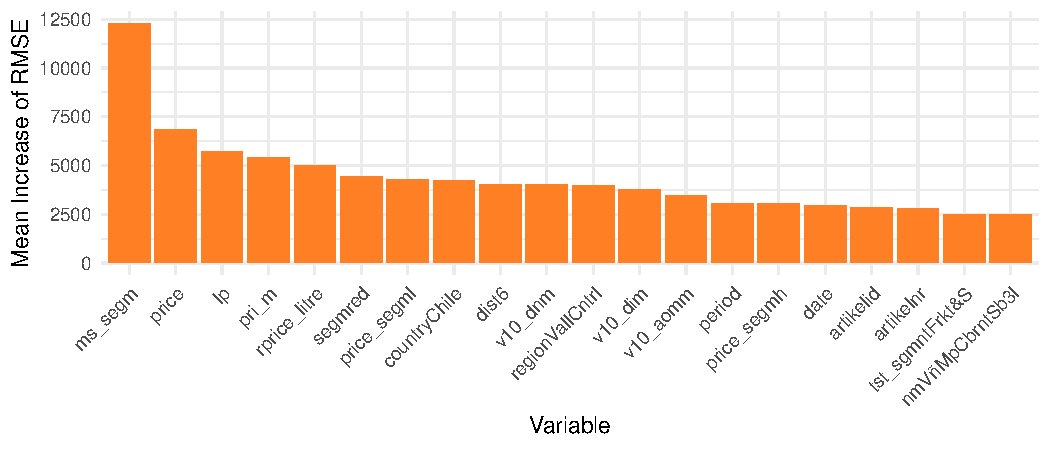
\includegraphics{../00_data/output_paper/11_var_imp_random_forest_bp.pdf}
\caption{Random Forest: Variable Importance.}
\end{figure}

\hypertarget{boosting}{%
\subsubsection{Boosting}\label{boosting}}

\begin{figure}

{\centering 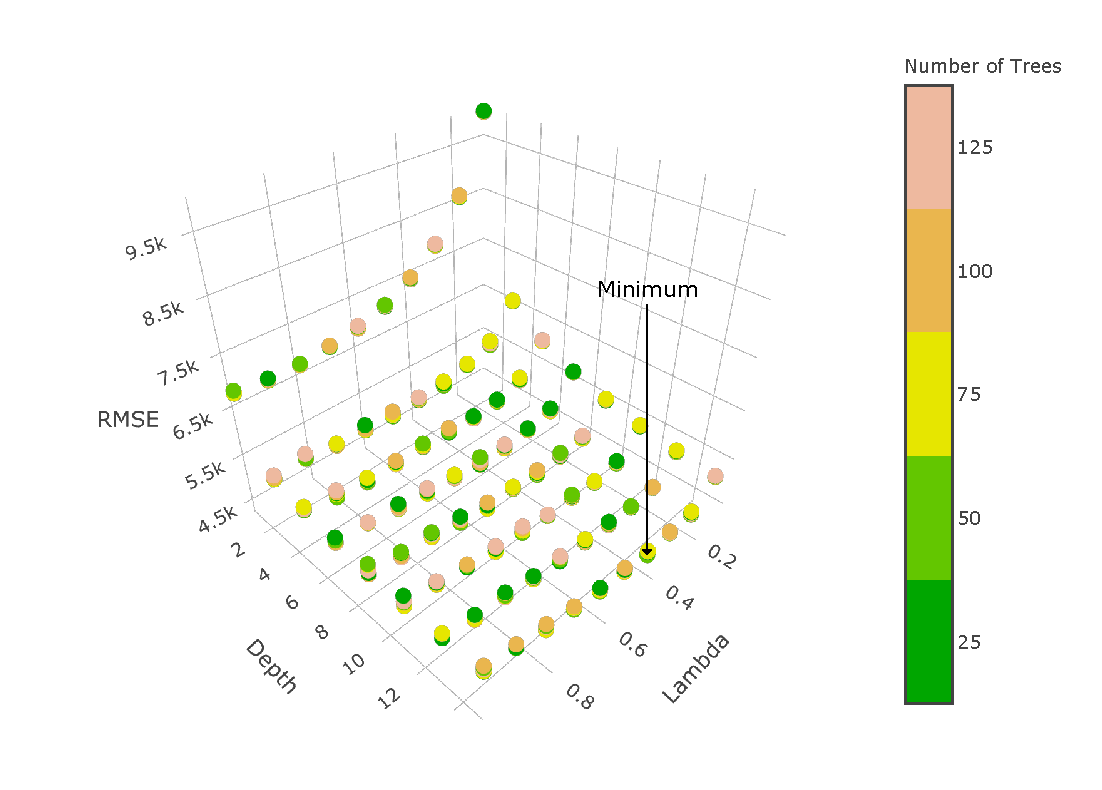
\includegraphics{../00_data/output_paper/11_boosting_plot} 

}

\caption[RMSE's of the Boosting Model for Different Parameters]{Boosting: Dependency between RMSE, Lambda, the Depths and the Number of Trees that are Grown.}\label{fig:boosting_hyper}
\end{figure}

In contrast to random forests boosting grows tree sequentially meaning
that for every new tree information from already grown trees is used
\autocite[cf.][p. 322]{James2014}. For boosting rather small regression
trees are used to improve the boosting tree slowly. This is achieved by
taking the residuals from the current boosting tree, fitting a (small)
tree to these residuals and then fiiting this tree into the boosting
tree in areas where the performance of the boosting tree could be
improved \autocite[cf.][p. 322]{James2014}.

\begin{figure}
\centering
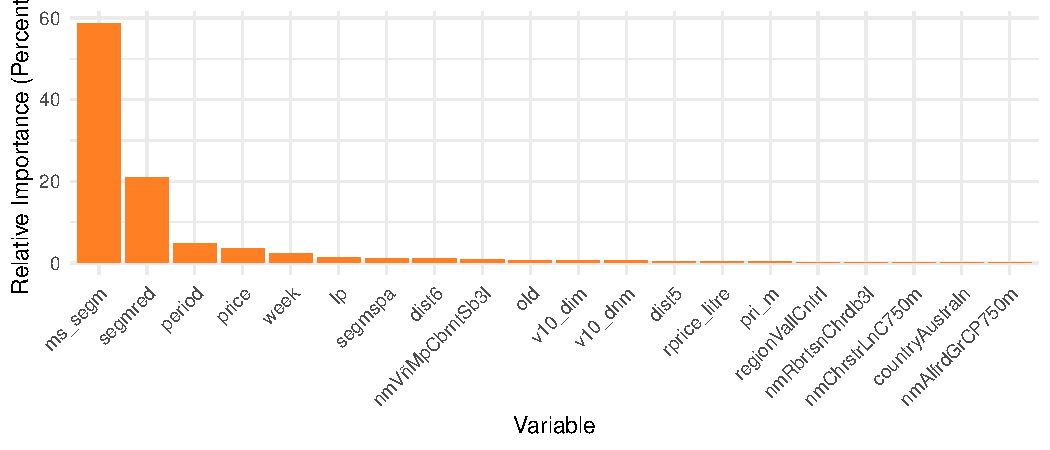
\includegraphics{../00_data/output_paper/12_var_imp_boosting_bp.pdf}
\caption{Boosting: Variable Importance Plot.}
\end{figure}

bag.fraction eklären! Wir nutzen hier jeweils 100\% unserer Observations
da dies optimal ist. Man kann es aber tunen. Siehe Zeile 328 im 00er
script

\hypertarget{conclusion}{%
\section{Conclusion}\label{conclusion}}

In this paper we tried to find an acurate forecasting model based on the
friberg gringvist wine data set. To achieve this goal we used different
techniques from the field of statistical learning methods and compare
those in terms of their mean RMSE (averaged over all folds of the
cross-validation). For comparison we set the RMSEs of the mean
regression and the simple linear regression as two baseline. The RMSE
obtained from the mean regression is \(\approx 7936\) litres sold per
week, which is a rather high value. This becomes clear when comparing it
to the mean RMSE of the linear regression model which is
\(\approx 6495\). This shows that the linear regression gives in basic a
better forecast than the mean regression, which probably is due to the
many more variables included in the linear regression.

\pagebreak

\addcontentsline{toc}{section}{References}
\printbibliography[title = References]
\cleardoublepage

\begin{refsection}
\nocite{R-base}
\nocite{R-broom}
\nocite{R-dplyr}
\nocite{R-ggplot2}
\nocite{R-haven}
\nocite{R-lmtest}
\nocite{R-PerformanceAnalytics}
\nocite{R-rstudioapi}
\nocite{R-sandwich}
\nocite{R-stargazer}
\nocite{R-svMisc}
\nocite{R-tidyr}
\nocite{R-xts}
\nocite{R-Studio}
\printbibliography[title = Software-References]
\addcontentsline{toc}{section}{Software-References}
\end{refsection}

\cleardoublepage
\appendix
\setcounter{table}{0}
\renewcommand{\thetable}{A\arabic{table}}

\hypertarget{appendices}{%
\section{Appendices}\label{appendices}}

\hypertarget{some-appendix-1}{%
\subsection{Some Appendix 1}\label{some-appendix-1}}

\newgeometry{top=1cm, left = 5cm, right = 2.5cm, bottom = 2cm}

\begin{table}[!htbp] \centering 
  \caption{Summary Statistics of the Data Set.} 
  \label{} 
\begin{tabular}{@{\extracolsep{5pt}}lcccc} 
\\[-1.8ex]\hline 
\hline \\[-1.8ex] 
Statistic & \multicolumn{1}{c}{Min} & \multicolumn{1}{c}{Max} & \multicolumn{1}{c}{Mean} & \multicolumn{1}{c}{St. Dev.} \\ 
\hline \\[-1.8ex] 
artikelnr & 200,001 & 4,236,201 & 1,008,268.000 & 847,223.200 \\ 
artikelid & 2,000 & 42,362 & 10,082.660 & 8,472.232 \\ 
year & 2,002 & 2,006 & 2,003.849 & 1.157 \\ 
week & 1 & 53 & 26.655 & 15.464 \\ 
period & 1 & 215 & 123.181 & 60.995 \\ 
litre & 0.000 & 184,200.000 & 6,100.028 & 11,361.840 \\ 
llitre & $-$0.288 & 9,999,979.000 & 6,357,811.000 & 2,766,722.000 \\ 
price & 38 & 1,149 & 109.710 & 86.164 \\ 
lp & 4,199 & 7,350,033 & 4,224,377.000 & 1,374,042.000 \\ 
rprice\_litre & 43 & 9,997,986 & 4,786,868.000 & 3,294,301.000 \\ 
old & 0 & 6,294 & 1,013.839 & 1,670.369 \\ 
ma\_split & 0.000 & 9,992,891.000 & 103,908.700 & 731,760.500 \\ 
v10\_a & 0.000 & 9,996,812.000 & 139,915.000 & 839,263.000 \\ 
v10\_dn & 0.000 & 1.000 & 0.866 & 0.341 \\ 
v10\_di & 0.000 & 6,666,667.000 & 700,363.200 & 1,870,385.000 \\ 
v10\_exp & 0.000 & 1.000 & 0.987 & 0.115 \\ 
v10\_svd & 0.000 & 1.000 & 0.983 & 0.130 \\ 
v10\_aom & 0.000 & 1.000 & 0.862 & 0.345 \\ 
v10\_am & 0.000 & 9,642,858.000 & 843,582.100 & 2,364,607.000 \\ 
v10\_dnm & 0.000 & 9,791,667.000 & 2,781,325.000 & 3,473,845.000 \\ 
v10\_dim & 0.000 & 9,642,858.000 & 2,152,525.000 & 3,281,604.000 \\ 
v10\_expm & 0.000 & 9,714,286.000 & 1,306,189.000 & 2,935,431.000 \\ 
v10\_svdm & 0.000 & 9,833,333.000 & 868,634.200 & 2,474,596.000 \\ 
v10\_aomm & 0.000 & 9,629,629.000 & 3,414,758.000 & 2,908,400.000 \\ 
v10\_all & 0.000 & 9,710,261.000 & 3,998,467.000 & 2,944,359.000 \\ 
rev\_all & 0.000 & 9,816,509.000 & 77,025.290 & 679,549.600 \\ 
rev\_all\_hi & 0 & 1 & 0.038 & 0.190 \\ 
rev\_all\_lo & 0 & 1 & 0.019 & 0.137 \\ 
rev\_eve & 0 & 1 & 0.015 & 0.122 \\ 
rev\_eve\_hi & 0 & 1 & 0.010 & 0.098 \\ 
rev\_eve\_lo & 0 & 1 & 0.003 & 0.058 \\ 
rev\_ex & 0 & 1 & 0.010 & 0.101 \\ 
rev\_ex\_hi & 0 & 1 & 0.008 & 0.089 \\ 
rev\_ex\_lo & 0 & 1 & 0.006 & 0.079 \\ 
rev\_nyaom & 0 & 1 & 0.033 & 0.179 \\ 
rev\_nyaom\_hi & 0 & 1 & 0.029 & 0.169 \\ 
rev\_nyaom\_lo & 0 & 1 & 0.013 & 0.113 \\ 
rev\_all\_p50 & 0 & 1 & 0.024 & 0.152 \\ 
rev\_all\_p80 & 0 & 1 & 0.017 & 0.130 \\ 
rev\_all\_p20 & 0 & 1 & 0.010 & 0.101 \\ 
m\_rev & 0 & 1 & 0.009 & 0.094 \\ 
m\_rev\_hi & 0 & 1 & 0.003 & 0.058 \\ 
m\_rev\_lo & 0 & 1 & 0.001 & 0.031 \\ 
nrarom & 0 & 793 & 14.917 & 74.440 \\ 
pri\_m & 0 & 9,990,796 & 3,046,590.000 & 3,513,496.000 \\ 
ms\_segm & 0 & 9,984,732 & 1,846,902.000 & 3,136,838.000 \\ 
ind & 0.00000 & 1.000 & 0.014 & 0.097 \\ 
...59 & 1.000 & 1.000 & 1.000 & 0.000 \\ 
\hline \\[-1.8ex] 
\end{tabular} 
\end{table}

\restoregeometry

\newpage
\textbf{Eidesstattliche Versicherung}

\bigskip

Ich versichere an Eides statt durch meine Unterschrift, dass ich die vorstehende Arbeit selbständig und ohne fremde Hilfe angefertigt und alle Stellen, die ich wörtlich oder annähernd wörtlich aus Veröffentlichungen entnommen habe, als solche kenntlich gemacht habe, mich auch keiner anderen als der angegebenen Literatur oder sonstiger Hilfsmittel bedient habe. Die Arbeit hat in dieser oder ähnlicher Form noch keiner anderen Prüfungsbehörde vorgelegen.

\vspace{1cm}
\rule{0pt}{2\baselineskip} %
\par\noindent\makebox[2.25in]{\indent Essen, den \hrulefill} \hfill\makebox[2.25in]{\hrulefill}%
\par\noindent\makebox[2.25in][l]{} \hfill\makebox[2.25in][c]{Jonathan Berrisch, Timo Rammert}%


\end{document}
